\documentclass[10pt,conference, compsocconf]{IEEEtran}

%\usepackage[ruled]{algorithm} \renewcommand{\algorithmcfname}{ALGORITHM}
%\SetAlFnt{\small} \SetAlCapFnt{\small} \SetAlCapNameFnt{\small}
%\SetAlCapHSkip{0pt} \IncMargin{-\parindent}
\usepackage{cite}
\usepackage[dvips]{graphicx}
\usepackage{algorithm}
\usepackage{algpseudocode}
\usepackage{pifont}
%---------------------------usepackages----------------------------
\usepackage{graphicx}
\usepackage{subfig}
\usepackage{makeidx}
%\usepackage{algpseudocode}
\usepackage{array}
\usepackage{multirow}
\usepackage{fancyhdr}
\usepackage{lastpage}
\usepackage{float}
\usepackage{booktabs}
\usepackage{url}
\newcommand\du{\mathrm{d}}
\usepackage{amsmath}
\usepackage{amssymb}
\usepackage{placeins}
\usepackage{mathrsfs}
\usepackage{CJKutf8}
%\usepackage{utf8x}{inputenc}
\usepackage[margin=2cm]{geometry}
\usepackage[utf8]{inputenc}
\usepackage{enumerate}
\usepackage[colorlinks=false]{hyperref}
\newcommand\relphantom[1]{\mathrel{\phantom{#1}}}

\pagestyle{fancy}
\fancyhf{}
\rfoot{\thepage}
%%--------------------------THEOREMs------------------------------
\newtheorem{thm}{Theorem}[section]

\let\definition\undefined
\let\lemma\undefined
\let\claim\undefined
\let\corol\undefined
\let\propos\undefined
\let\rema\undefined
\newtheorem{definition}{Definition}
\newtheorem{lemma}[thm]{Lemma}
\newtheorem{claim}[thm]{Claim}
\newtheorem{corol}[thm]{Corollary}
\newtheorem{propos}[thm]{Proposition}
\newtheorem{rema}{Remark}[section]
\def\bde{\begin{definition}}
\def\ede{\end{definition}}
\def\bp{\begin{propos}}
\def\ep{\end{propos}}
\def\bt{\begin{thm}}
\def\et{\end{thm}}
\def\bco{\begin{corol}}
\def\eco{\end{corol}}
\def\bl{\begin{lemma}}
\def\el{\end{lemma}}
\def\br{\begin{rema}}
\def\er{\end{rema}}
\def\be{\begin{equation}}
\def\ee{\end{equation}}
\def\ba{\begin{array}}
\def\ea{\end{array}}
\def\bena{\begin{eqnarray}}
\def\eena{\end{eqnarray}}

%-------------------------------Letter ab.------------------------
\def\P{{\mathbb P}}
\def\E{{\mathbb E}}
\def\R{{\mathbb R}}
\def\Z{{\mathbb Z}}
\def\N{{\mathbb N}}
\def\Q{{\mathbb Q}}
%\def\1{\mathbbold{1}}
\def\1{I}
%%%--------------------
\def\fA{{\cal A}}
\def\fB{{\cal B}}
\def\fC{{\cal C}}
\def\fD{{\cal D}}
\def\fE{{\mathscr E}}
\def\fF{{\mathscr F}}
\def\fG{{\mathscr G}}
\def\fK{{\mathscr K}}
\def\fL{{\mathscr L}}
%--------------------
\def\ze{{\zeta}}
\def\nb{{\nonnumber}}
\def\lb{{\label}}
\def\la{{\lambda}}\def\La{{\Lambda}}
\def\ga{{\gamma}}\def\Ga{{\Gamma}}
\def\a{{\alpha}}
\def\d{{\delta}}\def\D{{\Delta}}
\def\o{{\omega}}\def\O{{\Omega}}
\def\var{\hb{Var}}

%------------------------------OTHERS------------------------------------
\def\QED{\hfill$\square$\vskip 3mm}
\def\qed{\vskip -22pt \QED}
\def\Dp{\displaystyle}
\def\Df{\Dp\frac}
\def\hb{\hbox}
\def\({\left(}
\def\){\right)}
\def\[{\left[}
\def\]{\right]}
\linespread{1}
 \date{}
%\usepackage{amsthm}
%\newtheorem{theorem}{Theorem}
% Metadata Information \acmVolume{0} \acmNumber{0} \acmArticle{0} \acmYear{xxxx}
% \acmMonth{0}

% Copyright %\setcopyright{acmcopyright} %\setcopyright{acmlicensed}
%\setcopyright{rightsretained} %\setcopyright{usgov} %\setcopyright{usgovmixed}
%\setcopyright{cagov} %\setcopyright{cagovmixed}

% DOI \doi{0000001.0000001}

%ISSN \issn{1234-56789}

\begin{document}
\begin{CJK}{UTF8}{gkai}

\title{A  Weight-based Approach to Combinatorial Test
  Generation for Higher Fault-detection Rate}

\author{\IEEEauthorblockN{Jing Zhao$^1$, Gao-Rong Ning $^3$, K-Y Cai $^3$, Zhiqiang Zhang $^5$,  Jian Zhang $^5$}
\IEEEauthorblockA{$1$ Department of Computer Science and Technology, Harbin Engineering University,
China, zhaoj@hrbeu.edu.cn \\
$3$ Department of Automatic Control, Beihang University, China, ninggaorong@asee.buaa.edu.cn \\
$4$ Department of Electrical and Computer Engineering, Duke University, USA, kst@duke.edu \\
$5$ The State Key Laboratory of Computer Science, Institute of Software, Chines Academy of Sciences, zhangzy@ios.ac.cn, China}
}

 \maketitle
\begin{abstract}
\emph{Combinatorial testing} (CT) is very efficient to test parameterized systems.
Kuhn et al. investigated the interaction faults of some real programs, 
and found that the faulty combinations are caused by the combination of 
no more than 6 parameters. 
Three or fewer parameters triggered a total of almost 90\% of the 
failures in the application\cite{Hagar2015computer}.
However, for high quality software,
simply testing all 3-way combinations is not sufficient \cite{kuhn02SEW},
which may increase the risk of residual errors that lead to system failures and 
security weakness\cite{Kuhn2010NIST}. 
In addition,
the test cases at 100\% percentage coverage for high-way are huge, which surpass farthest 
for the test cost restrictions.
\emph{covering array} is typically used as the test suite in CT, 
which should convey much information for the fault detection, 
We firstly proposed a weighed combinatorial coverage,
focusing the fault detection capability of each test case instead of
100\% percent \emph{t}-way combinatorial coverage.
Secondly, we give the test case selection algorithm using 
weighted combinatorial coverage metric. 
For generating each test case, 
our method first randomly generates several candidates,
and selects the one that has the highest fault-detection possibility. 
Thirdly, we give the theorem for our algorithm and definitions for the 
weighted combinatorial coverage. 
Finally, we develop the simulation model to prove that our algorithm 
efficiency with varying candidate test case size. 
\end{abstract}


\begin{IEEEkeywords}
combinatorial testing; weighted combinatorial coverage; fault detection rate ; test case selection; simulation 
\end{IEEEkeywords}
%\keywords{Combinatorial testing, test generation, covering array, weight-based
%fault-detection-rate}

%\begin{bottomstuff}
%\end{bottomstuff}


\section{Introduction} Since the 21st century, computer software has been more
and more involved in people's life. As software is created by humans, it may
have defects. The harm brought by defective software varies from undetectable
minor problems to catastrophic accidents such as economic losses, equipment
failures or even life endangerment
\cite{tassey02NIST,ariane5,leveson93Computer}.  Software testing is a common way
of ensuring software quality. Although software testing cannot guarantee the
system under test (SUT) is error-free, a good testing practice can help detect
many defects in the SUT, and provide higher confidence.

There are many software testing techniques, each of which is suits for some
circumstances. \emph{Combinatorial testing} (CT) is one of these techniques,
which is very efficient to test parameterized systems.
In CT, the SUT is modeled as a black-box,
whose behavior is affected by several input parameters (or
called parameter/configurations).
Each parameter may take several possible values.
From a black-box view, the failures are caused by the combination
effects of parameters.
These faults are called \emph{interaction faults}.
These failure-causing parameter combinations are called \emph{faulty combinations}.
Without any a priori knowledge, any parameter combination may
be faulty.
In the worst case, we need to test all possible parameter combinations,
in which the number of test cases increases exponentially with the
number of parameters.
The number of \emph{t}-way tests that will be required is proportional to
 $v^t \log n$, 
for $n$ parameters with $v$ values each
\cite{Kuhn2010NIST,Cohen1997TSE}. 
Kuhn et al. \cite{kuhn02SEW,kuhn04TSE,Hagar2015computer} investigated the interaction faults of
some real programs, and found that the faulty combinations they studied are caused by 
the combination of no more than 6 parameters.
Empirical investigations have concluded that from 70\% to 90\% of the failures
could be identified by pairwise combinatorial testing\cite{kuhn04TSE}.
This point can also be supported by other studies \cite{zhang11ISSTA,vilkomir13ICSTW}.
If we have tested all small parameter combinations (e.g. all 3-way combinations),
we can detect many interaction faults,
three or fewer parameters triggered a total of almost 90\% of the 
failures in the application\cite{Hagar2015computer}.
However, for high quality software,
simply testing all 3-way combinations is not sufficient \cite{kuhn02SEW},
which may increase the risk of residual errors that lead to system failures and 
security weakness\cite{Kuhn2010NIST}. 

In CT, we typically use \emph{covering arrays} (CA) as the test suite.
%We give
%an appropriate covering strength $t$, and generate a CA of strength $t$, which
%covers all $t$-way parameter combinations. Then we can find failures caused by
%$t$-way parameter combinations.
%A notable fact is that, a $t$-way covering arrays also cover parameter
%combinations greater than size $t$, thus they may also detect some larger faulty
%combinations. Chen et al. \cite{chen11ICSE} proposed a metric for measuring the
%covering strength of a CA with a decimal fractions rather than an integer, by
%taking the coverage of $t+1$-way parameter combinations into consideration.
Looking back the typical way of doing combinatorial testing, we give the
covering strength in advance, specifying which combinations need to be covered
(we call them \emph{target combinations}), and generate a CA to cover all these
combinations.
Then the test generation is done. We use \emph{t}-way combinatorial coverage
as a metric to select the best coverage test case.
Which coverage criterion should be chosen or determined by the cost of test
and the quality requirement of the software. 
Suppose a Software Under Test(SUT) has 20 parameters, and each parameter has 10 
values, we can check all pairs of these values with only 180 tests by 
using pair-wise coverage, 
if \emph{N}-way coverage used then $10^{20}$ test
cases will be used which is far more than a software tester would be 
test in a lifetime \cite{Kuhn2009computer}.
For finding the remaining faults,
one way is to change the \emph{t}-wise coverage criterion. 
if we change the coverage criterion from pair-wise to 5-wise, Almost all the faults
can be found by using 100\% percentage coverage. Furthermore, if we employ 6-wise 
combinatorial coverage, the testing process will be forced to stop at a large SUT 
because the test cases at 100\% percentage coverage are huge, which surpass farthest 
for the test cost restrictions.
The problem is that we focus too much on the target combination. 
%The problem is, we are focusing
%too much on the target combinations. Actually, the reason why we choose a
%covering strength $t$ in advance is that most faulty combinations are small, and
%if we select an appropriate $t$, then we can detect most of the defects.
%However, 

In software testing,
we should consider test effectiveness as well as efficiency for a SUT. 
And the efficient test case require that the generated test case 
should contribute much useful information which can be use to 
find faults in the SUT.
we usually want to detect as many defects with as
less cost as possible, and also to detect defects as early as possible.
For this need, the fault-detection rate of the test suite is important. 
In CT, we usually use the cover array to represent a test case.
Thus, a covering array should convey much information for the fault detection, 
and we shift our focus from \emph{t}-way combinatorial coverage 
to the fault-detection possibility of each test case.
We measured the exposed average faults by executing every test case,
in which the faults will be 1-way, 2-way,..., 6-way, etc. 
%We use the \emph{t}-way ratio that estimated \emph{t}-way faults divide by the sum of the faults as
A \emph{t}-way combinatorial coverage weight can be calculated based on 
presumed distribution of faulty combination size.
Therefore, the combinatorial coverage can be regarded as the sum of the 
weighted \emph{t}-way coverage.
Thus, Combinatorial testing focus on generating the optimized 
test case that has the highest fault detection rate, 
instead of selecting at 100\% percentage combinatorial coverage.

%Combinatorial testing include the static testing, dynamic testing like general testing process.
%As for the static testing, testers need to determine the parameters which do
%not change during the testing process. Although static testing is simple, it 
%depend on the parameter settings. While dynamic testing can tune up the values of 
%parameters as test cases executed. In this paper, we consider both static 
%testing and dynamic testing.
Our approach is based on the one-test-at-a-time strategy.
For generating each test case, our method first randomly generates several
candidates, and selects the one that has the highest fault-detection
possibility. The fault-detection ability is calculated based on the
presumed distribution of faulty combination size, 
which could be given in advance based on one's experience and knowledge about the SUT. 
The traditional way of CT is
a special case of our method where all faulty combinations are of size $t$,
which requires choosing the covering strength first,
if the strength is set too large that resources will be wasted or forced 
to stop, or if the strength is set too small that the covering array  
is insufficient to find the specific failures\cite{Nie2013QSC}.  

%Although we know the test suite may detect larger faulty combinations,
%existing test generation
%algorithms only focus on the $t$-way combinations.

In summary, our main contributions are as follows:

\begin{itemize}
 \item We propose the metric of weighted combinatorial coverage, 
 which connect the combinatorial coverage and the fault detection 
 capability of each test case.
 \item We propose an algorithm for the weighted combinatorial
 test case selection, and it is theoretically proved that our algorithm
 efficiency with varying candidate test case size.   
 \item We develop a simulation model to prove that our algorithm 
 efficiency with varying candidate test case size. 
\end{itemize}
%Thus, the presumed t-way fault detection rate can be obtained accordingly. 
%For static testing of combinatorial, the presumed t-way fault detection rate
%do not change during the testing process.  Alternatively,for dynamic combinatorial
%testing, we
%provide an adaptive version of algorithm, which can dynamically update fault detection
%rate based on the execution result of test cases, and the testing process is 
%a closed feedback.  
%The algorithm requires
%the tester to execute each test case after it is generated.
%If the test fails,
%then it uses CT-based fault localization techniques to locate the faulty
%combination and updates the distribution of faulty combinations.
%
%Experimental results show that: ...
This paper is organized as follows. In section \ref{sec:relatework},
we give the related work for combinatorial testing.
In section \ref{sec:weight definition},
we first give a motivation example for our approach, and next 
we give the definition for weighted combinatorial coverage, 
and we prove the theorem that combinatorial coverage rate 
equals to the fault detection rate. In section \ref{sec:algorithm},
we give an algorithm for weighted combinatorial test case selection, 
and give the theorems for proving algorithm efficiency. In section \ref{sec:exp}, 
we did the simulation to check the efficiency for our algorithm. 
In section \ref{sec:conclustion}, we give the conclusion for the paper. 

\section{Related Work}
\label{sec:relatework}
Typically, to apply CT to a system under test requires the following steps:

\begin{itemize}
\item Modeling: building a parameterized model for the SUT which is suitable for
later test generation. The tester identifies the parameters (factors) that
affects the SUT behavior according to the specification and test goal. Then s/he
needs to identify the possible values for each parameter, as well as the
covering requirement;

\item Test generation: generating a covering array according to the SUT model
and covering requirement;

\item Test prioritization and reduction: postprocessing of the covering array.
Test prioritization mainly focuses on reordering the test cases for early fault
detection, while test reduction aims at modifying the test suite to reduce
number of test cases while still preserving the coverage;

\item Test execution: to run test cases on the SUT and observe the results;

\item Fault localization: locating the faulty combinations that caused some test
cases to fail during the test execution process.
\end{itemize}

Orthogonal arrays and covering arrays are usually popularly used 
as combinatorial design\cite{Mats2005testing}.
Zhang et al. \cite{zhang14book} wrote
a book which surveyed the major approaches to this topic. Existing methods can
be classified into mathematical construction methods and computational methods.

Mathematical construction methods are usually based on mathematical theories,
and they usually know what the CA should be look at in advance.
However, the main drawback of these approaches is that their method is
not very limited, they can hardly deal with some real testing requirements such
as mixed-level covering array (parameters have different number of values),
variable strength and constraints.

Different from mathematical construction methods, computational
methods does now know what the covering array should be look like. They focus on
the coverage requirement, and try to adjust the array to cover more and more
target combinations.
Computational methods can be
categorized into three types of methods\cite{nie11CSUR} based on how they fill entries in the
array.
The first type of computational methods are based on the one-test-at-a-time
strategy\cite{kuhn13book}. Algorithms of this strategy generates the CA row-by-row, which means
that they iteratively generate new test cases and add it into the array, until
all target combinations are covered. For generating each test case, these
algorithms try to find a test case that covers the greatest number of uncovered
test cases. The differences between these algorithms is that they use different
strategies to optimize the new test case\cite{sherwood94STAR}
The AETG algorithm
generates each new test case by first generating several candidates and then
selecting the one that covers the greatest number of uncovered test cases.  For
generating each candidate test case, it greedily assign values to parameters in
a random order. Some other AETG-like algorithms include TCG \cite{tung00AC} and
mAETG-SAT \cite{cohen07ISSTA,cohen08TSE}. PICT \cite{czerwonka06PNSQC} generates
each new test case by assigning parameters one by one. Each time it greedily
selects a parameter-value pair to assign.  The deterministic density algorithm
(DDA) generates a new test case using a density-based method, where the density
is computed based on the uncovered target combinations. The method by Clavagna
and Gargantini \cite{calvagna08TAP} generates each new test case by greedily
selecting a set of consistent uncovered target combinations to assign some of
the parameters, and using a model checker to find values for the remaining
parameters. Cascade \cite{zhao13ICSTW,zhang14JSS} converts the problem of
generating a new test case into a pseudo-Boolean algorithm, and calling an
optimizations solver to find a solution. There are also some other
one-test-at-a-time approach based on meta-heuristic search algorithms, such as
simulated annealing, hill climbing, genetic algorithm, ant colony algorithm,
tabu search, great flooding and particle swarm optimization
\cite{shiba04COMPSAC,bryce07GECCO,ahmed11JSS,ahmed12ASC}.

The second type of computational methods are IPO-based algorithms \cite{lei08STVR}.
Different from the one-test-at-a-time strategy, which expands the array only
vertically, IPO-based algorithms expands the array both vertically and
horizontally. These algorithms starts from a small covering array, and
continuously extends it into a larger array.
The third type of computational methods are based on the whole-array-search
strategy. These algorithms try to generate a covering array of a given size,
which means the number of rows and columns are fixed in advance, and they need
to find an assignment to each entry to meet the coverage requirement. Hnich et
al. translated the properties of a covering array into SAT constraints, and use
a SAT solver to find a feasible solution. CASA \cite{garvin09SSBSE,garvin11ESE} used simulated annealing
to maximize the number of covered target combinations. If all target
combinations are covered, then the array is a covering array.

Like many test case selection methods, combination strategies are based on coverage\cite{Mats2005testing}.
Each-used coverage is the simplest coverage criterion. $100\%$ each-used coverage
requires that every interesting value of every parameter is included in at least 
one test case in the test suite. $100\%$ pair-wise coverage requires that possible
pair of interesting values of two parameters are included at each teat case in the 
test suite. A natural extension of pair-wise coverage is \emph{t}-wise coverage, of which,
A special case of \emph{t}-wise coverage is \emph{N}-wise coverage.
Which cover array should be adopted is determined by the size and quantity expected of the SUT.
For example, Grindal\cite{Mats2005testing} evaluated 
5 combination strategies: AC, EC, BC, OA and PW.
After the cover array is determined, then the test effort is to improve the coverage. 
For the Heuristic pair wise testing, at each step, the test
is to select that covered most pairs. 
The current CT approach intended to change the coverage criteria by 
improving the \emph{t}-wise criteria. The size of an test set grows 
logarithmically in the number of test parameters\cite{Cohen1997TSE},
In practice, test engineers faced with the deadlines and expensive 
long period testing processes, so high wise combinatorial testing
may not satisfy the testing requirements.
Fochen et.al proposed an incremental covering array failure 
characterization in large configuration space\cite{Fouche2009ISSTA},
which begins at the lower strength and then iteratively 
increases strength as resources allow. 
This approach's target is to find the faults as early as possible. 
However, this approach did not quantitatively reveal the 
fault detection capability with the used \emph{t}-way covering array,

Another way is the test prioritization process,
which improve the fault detection rate at early
stage by defining appropriate coverage metric.
Many of the current research employ the test prioritization technique,
which re-order the test suits to improve the early coverage.
Test prioritization focuses on the execution order of test cases by determining
the coverage metric that is used to select cover array.
Some approaches reorders the test cases for early fault detection
\cite{qu07ICSM,qu08ISSTA,qu13ICSTW}. Bryce and Colbourn \cite{bryce06IST}
adapted the DDA algorithm to prioritize test cases using user-specified weights
on parameters, values or combinations.
Elbaum et.al give the prioritization technique for the specific modified
version, and the correspondingly metric for fault detection rate APFD 
is proposed to measure the fault detection rate.
Some other approaches reorders the test
cases to minimize the switching cost (i.e. the cost of switching the current
test case to the next one) \cite{kimoto08SSIRI,srikanth09ISSRE,wu14ICSTW}.


Our method focuses on detecting faults at early stage by defining
weighted combinatorial coverage metric.
The user need to provide the presumed distribution of the faulty
combination size. However this distribution highly depends on the SUT itself and
the model.  Some empirical studies applied CT to different types of systems, and
evaluated the effectiveness of CT at different covering strength, as well as the
distribution of faulty combination sizes in the subject systems. In the study by
Kuhn et al. \cite{kuhn02SEW,kuhn04TSE}, they found that in their systems under
investigation, most faulty combinations are small, and their size is smaller
than 6. Some studies on other programs also found similar results
\cite{zhang11ISSTA,vilkomir13ICSTW}. 


\section{The weighted combinatorial coverage paradigm}
\label{sec:weight definition}
Consider the problem of testing a object software like Siemens suit(ref) which may
be injected faults, such as 1-way faults, 2-way faults, ...,6-way faults. 
We will give the motivation for the weighted combinatorial testing. 
\subsection{Motivation}
Assume that the software testers know in advance that each $i_{way}$ faults 
existed in the testing suit by their testing experiences.
We assume that the presumed distribution of each $i_{way}$ faults are as the follows out of the 
total faults being $n$:
1-way faults $n*20\%$, 2-way faults $n*35\%$, 3-way faults $n*25\%$, 4-way faults $n*10\%$,
5-way faults $n*5\%$, and 6-way faults $n*5\%$.
Let the Card($V_t$) denote the cardinality of t-way combinations, i.e., 
the number of t-way combinations for the object system.
So that, we can give each t-way fault detection rate as follows:
$e_1=\frac{n*20\%}{Card(V_1)}$, 
$e_2=\frac{n*35\%}{Card(V_2)}$, 
$e_3=\frac{n*25\%}{Card(V_3)}$, 
$e_4=\frac{n*10\%}{Card(V_4)}$, 
$e_5=\frac{n*5\%}{Card(V_5)}$, and
$e_6=\frac{n*5\%}{Card(V_6)}$. 
The expected detection faults for each test case can be calculated by the weighted 
combinatorial coverage. Assume that the $m^{th}$ test case is employed to test the system, 
and the new added t-way combinations for the $m^{th}$ test case are $c_t$ (t=1,2,3,4,5,6).
Then, we can obtain the expected detection faults by calculating $\sum_{t}{e_t\cdot{c_t}}$. 
%Whatever the static combinatorial testing or dynamic combinatorial testing,
Both in static combinatorial testing and in dynamic combinatorial testing,
we can select the test case that the estimated expected faults are highest. 
Next, we first give the definitions for the $i_{way}$ combinatorial coverage rate, and 
then we give the definition for the weighted combinatorial coverage rate. 
\subsection{Definition for weighted combinatorial coverage rate} 

Definition 1:
$i_{way}$ combinatorial coverage: 
Assume $m_{i}(t)$ denote the total $i_way$ combinations used when the $n_{th}$ test case 
finished testing, and $M_{i}$ denote the total $i_{way}$ combinations. Then, the $i_{way}$ 
combinatorial coverage, $\rho_{i}(t)$, can be defined as: 
$\rho_{i}(t)=\frac{m_{i}(t)}{M_{i}}$

Definition 2:
Weighted combinatorial coverage:
Based on the $i_{way}$ combinatorial coverage, $\rho_{i}(t)$, the weighted combinatorial coverage,
$\rho(t)$, can be defined as:

\begin{equation}
\label{weighted_combinatorial_original}
\rho(t)=\rho_{i}(t)\cdot{\frac{\hat{b}_i(t)}{\sum_i{\hat{b}_i(t)}}}
\end{equation}
where $\hat{b}_i(t)$ denotes that estimated $i_{way}$ faults in the system
when the $n^{th}$ test cases finished testing. 

\begin{thm}
The weighted combinatorial coverage rate, $\rho(t)$, which equals to the fault detection rate,
$\frac{\hat{b}_i(t)}{\sum_i{\hat{b}_i(t)}}$.
\end{thm}

PROOF. Consider that $\hat{b}_i(t)$ denotes the estimated total $i_{way}$ faults when the $n^{th}$ 
test case finished testing. We need to estimate the total $i_{way}$ faults since we did not know 
the number of faults at the beginning testing.
Then, the total faults for the system which include each $i_{way}$ is $\sum_i{\hat{b}_i(t)}$. 
According to the following formula, in which, $c_i(t)$ denotes the found faults using the 
number of $t$ test cases when the $t^{th}$ test case finished testing.
\begin{equation}
\label{fault_combination}
\frac{\hat{b}_i(t)}{c_i(t)}=\frac{M_i}{m_i^(t)}
\end{equation}
We can obtain
\begin{equation}
\label{estimate}
\hat{b}_i(t)=\frac{M_i}{m_i(n)}\cdot{c_i(t)}
\end{equation}
Then, we can input \label{estimate} into the weighted combinatorial coverage $\rho(t)$,
we obtain the following formula:
\begin{equation}
\label{weighted_combinatorial_equal}
\rho(t)=\frac{c_i(t)}{\hat{b}_i(t)}
\end{equation}
From (\ref{weighted_combinatorial_original}) and (\ref{weighted_combinatorial_equal}), 
we can deduce that the weighted combinatorial coverage rate $\rho(t)$ equals the
fault detection rate. Thus, we connect the weighted combinatorial coverage rate with
the fault detection rate.
Previous study compute the combinatorial coverage without considering the fault detection rate of individual test case. 
Given the short time availability during regression testing, a prioritization criterion that
is effective at selecting tests that detect faults quickly while at the same time, selects
tests that execute quickly would be highly beneficial. With this goal in mind, we modify the combinatorial
coverage metric to incorporate weighted fault detection rate of test cases. 

\section{Algorithm for weighted combinatorial test case selection}
\label{sec:algorithm}
\subsection{algorithm}
We incorporate the fault detection rate for $i_{way}$ faults into the $i_{way}$ combinatorial coverage,
then we define the weighted combinatorial coverage $\rho(t)$, which is the reasonable criteria in terms
of the improved fault detection rate.
Given the short time availability during regression testing, 
the weighted combinatorial coverage is effective at selecting tests that detect faults quickly.
Fig.\ref{alg:static} shows the weighted combinatorial coverage algorithm.
Firstly, we identify the parameters, values, and interactions. 
Next, we generate test case suit by the requirement,
and then we randomly select $m$ test cases from the generated test cases, where $m=5,10,15,20$. 
We select the "next test" that it expose the maximum expected number of faults, $w_{jx}$,
from $m$ selected test cases,  
which equals the total of 1-{way} faults, 2-{way} faults, ...etc. 

\begin{algorithm*}
\caption{weighted combinatorial coverage  algorithm}
\label{alg:static}
\begin{algorithmic}[1]
 \State $identify\ parameters,\  values,\ and\ interactions;$
 \State $Design\ test\  cases\  suit\  by\  requirements;$
 \State $1\leq\ i \leq N,\  1\leq\  k\  \leq m,\ j=1,\  S_{0i}=\emptyset, \ F_i=0$
    \While{$j\leq\ maximum\  number\  of\  cases\  or F_i\neq\ 0$}
         \State $Random\ select\ a\  test\  case\  from\  set\  t_{j1}, t_{j2},...,t_{ji},...,t_{jm};$ 
         \State $the\  weight\  of\  t_{jk}\  is\  w_{jk};$
         \State $w_{jk}=\vert {u_{j1k}}\vert \cdot e_1+\vert {u_{j2k}}\vert \cdot e_2+...\vert {u_{jik}}\vert \cdot e_i+...+\vert {u_{jNk}}\vert \cdot e_N;$ 
         \State $where\  u_{jik}=\{i-value\  slices\  in\  t_{jk}\  but\  not\  in\  S_{(j-1)i}\}$ 
         \State $w_{jx}=max(w_{jk});$ 
         \State $Let\  t_{jx}\  be\  the\  test\  case\  with\  largest\  w_{jx};$ 
         \State $\{u_{jix}, 1\leq i \leq N\}\  as\  the\  correspondingly\  new\  added\  combinations;$ ;
         \State $S_{ji}=S_{(j-1)i} \cup \{u_{jix, 1\leq i \leq N}\};$ 
         \If{find\  the\  failure}
                  \State $F_{i}=F_{i}-1$ 
         \Else                  
                   \State $Continue\  test;$
          \EndIf               
          \State $j=j+1;$
      \EndWhile 
 \end{algorithmic}
 \end{algorithm*}

\subsection{Theorem for Algorithm\ref{alg:static}}
 
\begin{thm}
\label{thm:thm2}
Let $B_i$ represent total i\_ways faults, and $M_i$ represent the number of i\_ways combinations.
Let $b_i(t)$ denote the number of faults for i\_ways combination when the $t$ test cases finished testing, 
and  $m_i(t)$ denote the used number of i\_ways combinations when the $t$ test cases finished testing.
The counting process $b_i(t),m_i(t)$ satisfy the following :
$\forall\varepsilon>0$,  
\begin{equation}
\label{equ:equ1}
\P\{|\frac{b_i(t)}{m_i(t)} - \frac{B_i}{M_i}| < \varepsilon \}\geq\ {1-\frac{1}{m_i(t)\cdot\varepsilon^2} }
%= \P\{|b_i(n)-\frac{B_i}{M_i}m_i(n)|) < \varepsilon \cdot m_i(n)\}
\end{equation}
\end{thm}

We consider $m_i(n)$ independent Bernoulli trials with the 
probability of finding failure equal to $\frac{B_i}{M_i}$ on each trial.
Thus, $b_i(n)$ follow $m_i(n)$ binomial distribution.  
Apply Chebyshev's inequality:
\begin{equation}
\label{equ:equ2}
\P(|X-E(X)| < \varepsilon) > 1 - \frac{D(X)}{\varepsilon ^ 2}
\end{equation}
Thus, the variance of $b_i(t)$ is $m_i(t) \cdot \frac{B_i}{M_i} \cdot (1-\frac{B_i}{M_i})$,
and the mean value of $b_i(t)$ is $m_i(t) \cdot \frac{B_i}{M_i}$. 
%将公式(9)中的$b_i(n)$看作是(8)中的$X$,\\
%        $\frac{B_i}{M_i} \cdot m_i(n)$看作是(8)中的E(X),$\varepsilon \cdot m_i(n)$看做是(8)中的$\varepsilon$,那么由(8)可知
Accordingly, we can obtain
\begin{equation}
\label{equ:equ3}
\P\{|b_i(t)-\frac{B_i}{M_i} \cdot m_i(t) \le \varepsilon \cdot m_i(t)\} \geq 1- \frac{M_i(t) \cdot \frac{B_i}{M_i}(1-\frac{B_i}{M_i})}{m_i(t)^2 \cdot \varepsilon^2}
\end{equation}
And also, from the equation \ref{equ:equ4},
\begin{equation}
\label{equ:equ4}
\frac{m_i(t) \cdot \frac{B_i}{M_i}(1-\frac{B_i}{M_i})}{m_i(t)^2 \cdot \varepsilon^2} \leq \frac{1}{m_i(t) \cdot \varepsilon^2}
\end{equation}
Therefore, we obtain the \ref{equ:equ5}
\begin{equation}
\label{equ:equ5}
1 - \frac{m_i(t) \cdot \frac{B_i}{M_i}(1-\frac{B_i}{M_i})}{m_i(t)^2 \cdot \varepsilon^2} \geq 1 - \frac{1}{m_i(t) \cdot \varepsilon^2}
\end{equation}
 Finally, we can prove the \ref{thm:thm2}.

\begin{thm}
\label{thm:thm3}
Assume that $b_i^{m_1}(t)$ and $b_i^{m_2}(t)$ are the faults detected
as the number of $t$ test case finished testing, 
when employing the optimized weight for Algorithm.1.
With the parameter $m=m_1,\ m_2$.
Let the expected detected faults with parameter $m=m_1,\ m_2$,
are $E(b_i^{m_1}(t))$, $E(b_i^{m_2}(t))$, respectively.
Thus, we have the following equation \ref{equ:equ6}
\begin{equation} 
\label{equ:equ6}
E(b_i^{m_1}(t)) \leq E(b_i^{m_2}(t))
\end{equation}
\end{thm}

when $t=1$, we select the best test case with the parameter $m=m_2$,
and the expected detected bugs are $E(b_i^{m_2})$. 
This process can be regarded as first randomly selecting the $m_1$ test
cases, in which we select the best case to detect the number of
$E(b_i^{m_1})$ $i-way$ faults.
And then we continue randomly select the $m_2-m_1$ test cases,
the expected number of detected bugs is $E(b_i^{(m_2-m_1)}(1))$.
While $E(b_i^{m_2}(1))=E(max\{b_i^{m_1}(1),b_i^{(m_2-m_1)}(1)\})$.
Thus, it is clearly that $E(b_i^{m_1}(1)) \leq\  E(b_i^{m_2}(1))$.

Assume $E(b_i^{m_1}(k)) \leq E(b_i^{m_2}(k))$ when $t\leq k$. 
We prove that when $t=k+1$ theorem\ref{thm:thm3} establish. 
We prove it by contradiction. 

First we let $E(b_i^{m_1}(k+1))\textgreater E(b_i^{m_2}(k+1))$,
algorithm find the number of faults 
$X_k$ when the number of $k$ test cases finished testing with $m={m_1}$.
And, $Y_k$ with $m=m_2$.
Then, we obtain the formula as follows: 
$$b_i^{m_1}(k)=\sum_{n=1}^{k}X_n,$$ and $$b_i^{m_2}(k)=\sum_{n=1}^{k}Y_n.$$
The expected detected bugs for the ${k+1}^{th}$ using the 
best selected case is $E(X(k+1)),E(Y(k+1))$ with 
parameter $m=m^1$ and $m=m^2$, respectively. 

We have already assumed that
$$E(b_i^{m_1}(k+1))\textgreater E(b_i^{m_2}(k+1)),$$i.e., 
$$E(b_i^{m_1}(k))+E(X(k+1)) > E(b_i^{m_2}(k))+E(Y(k+1)).$$

As for $E(X(k+1))$, we can regard $m_1$ as first select $m_0$ 
and then select $m_1\-m_0$. 
$E(X^{m_0}(k+1))$ denote the expected number of detected bugs
with $m^0$,and 
$E(X^{(m_1-m_0)}(k+1))$ denote the expected number of detected
bugs with   $m_1-m_0$. 
In which, 
$$E(X(k+1))=E(max \{X^{m_0}(k+1)),X^{(m_1-m_0)}(k+1))\} ).$$
For $m=m_2$, We employ the same approach as $m=m_1$. 
Thus, $$E(Y(k+1))=E(max \{Y^{m_2}(k+1),Y^{(m_2-m_0)}(k+1))\})$$ 
There exists a $m_0$, which make
$$E(b_i^{m_0}(k))+X(k+1) = E(b_i^{m_0}(k))+Y(k+1)$$
At the second phase of selecting, we have $m_1-m_0$,$m_2-m_0$.
Because $m^1-m^0<m^2-m^0$
so that we have $X^{(m_1-m_0)}(k+1)) \leq Y^{(m_2-m_0)}(k+1))$ ,
And also because
$$E(X(k+1)) =E(max \{X^{m_0}(k+1)),X^{(m_1-m^1_0)}(k+1))\} ),$$
$$E(Y(k+1)) =E(max \{Y^{m_0}(k+1)),Y^{(m_2-m^1_0)}(k+1))\} ),$$
Moreover, 
$$E(b_i^{m_1}(k))+X^{m_0}(k+1)) = E(b_i^{m_2}(k))+Y^{m_0}(k+1)),$$
i.e.,
$$E(b_i^{m_1}(k)) = E(b_i^{m_2}(k))+ (Y^{m_0}(k+1)) - X^{m_0}(k+1))).$$
Because,  
$$(Y(k+1)) - X(k+1)))\geq (Y^{m_0}(k+1)) - X^{m_0}(k+1)))$$
Thus,
$$E(b_i^{m_1}(k)) \leq  E(b_i^{m_2}(k))+(Y(k+1) - X(k+1))$$
i.e.,
$$E(b_i^{m_1}(k))+ X(k+1)) \leq E(b_i^{m_2}(k))+Y(k+1))$$
i.e.,
$$ E(b_i^{m_1}(k+1)) \leq E(b_i^{m_2}(k+1))$$
This contract with the assumption $ E(b_i^{m_1}(k+1)) \geq E(b_i^{m_2}(k+1))$
Therefore, $\forall n \leq  1 ,E(b_i^{m_1}(k)) \leq E(b_i^{m_2}(k)) $

Proof finished.

\section{Experiment}
\label{sec:exp}
We did the simulation to check the effectiveness of the static algorithm.
The input for the simulation model has 13 parameters, and the parameter
values is $\{4,2,6,7,3,6,2,3,10,4,5,5,3\}$. That is, the first parameter
had 4 values, the second parameter had 2 values, ..., and the last parameter
had 3 values. This gives a total of 108864000 combinations. 
We injected faults for $1_{way}$, $2_{way}$, ..., $6_{way}$ into the
simulation environment. And, the faults size for $i_{way}$ are denoted 
as $\{8, 65, 78, 68, 35, 1\}$.
For the testers experience, we employ the good weight that is used to denote 
the testers good experience for guessing the software faults for $i_{way}$. 
The employed good\_weight is $\{9,67,76,66,37,2\}$, 
and the bad\_weight is $\{10,170,70,8,0,0\}$.

%Since the pair-wise algorithm is popularly used algorithm.  
%$\{0,60,0,0,0,0\}$ denote as the 2-wise faults injected, 
%which can also be regarded as the bad\_weight for static algorithm.
In one simulation, we use good\_weight and bad\_weight parameter
to test the effectiveness of algorithm and compare between the
effectiveness between good\_weight and bad\_weight.
%In the simulation, we compare the  good\_wight with the pair-wise 
%algorithm. 
we compare the test effectiveness for 
different value settings when $m=5,10,20,40$, and we prove 
theorem\ref{thm:thm3} by using this application.  

In the simulation settings, the total injected faults are 255.
At each $m$ value, we have 20 runs using different seeds. 
Thus, at each fault of total 255, we calculate the mean value of 
20 runs. We obtain the test cases used for
good\_weight, bad\_weight, respectively.
Furthermore,
we obtain the combinatorial coverage, $i\_{way}$ coverage at good\_weight,
bad\_weight case. Next we give the metric for comparison. 
\subsection{Comparison Metric}
Metric\_1: $1\cdot{C_1}+2\cdot{C_2}+...+i\cdot{C_i}+...+N\cdot{C_N}$\\
Metric\_2: $C_1+C_2+...+C_N$\\
Metric\_1 denotes the number of detected faults(x-axis value)
multiply the number of tested cases(y-axis value),$C_i$. Or,
the number of tested cases (x-axis value) multiply the number of
detected faults(y-axis value).
Metric\_2 denotes the sum of the values of y-axis at fixed x-axis value. 

\subsection{Results}
Figure \ref{fig:gooda} shows that at the good\_weight case,
the x-axis denote the bug number, and the y-axis denote the number of
test cases used to detect the correspondingly bugs.
As shown in the Figure \ref{fig:gooda}
for example, $m=5: 20161026,1429$  and $87226.6429$ means that  
Metric\_1 value is 87226.6429, Metric\_2 value is 87226.6429.
The same meaning with $m=10,20,40$. 
The less y-axis value denote that the less test cases
used to detect the same amount of faults.  
Figure \ref{fig:bada} also shows when $m=40$,
the test efficiency is best, and then for $m=10$, $m=5$, 
and the last one is $m=20$.
The above figures are all enlarged parts.

 \begin{figure*}
 %[htb]
   \centering
   \subfloat[Algorithm 1:Good Distribution(enlarge)]{
   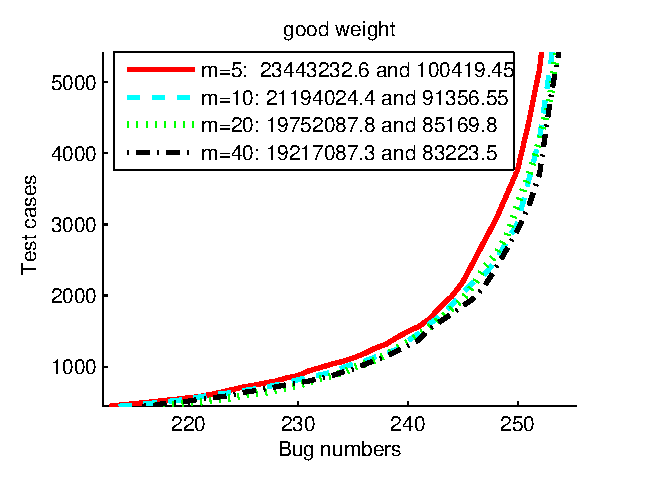
\includegraphics[width=0.45\textwidth]{./a1_picture_enlarge/good_enlarge.eps}
   \label{fig:gooda}
   }
   \subfloat[Algorithm 1:Bad Distribution(enlarge)]{
   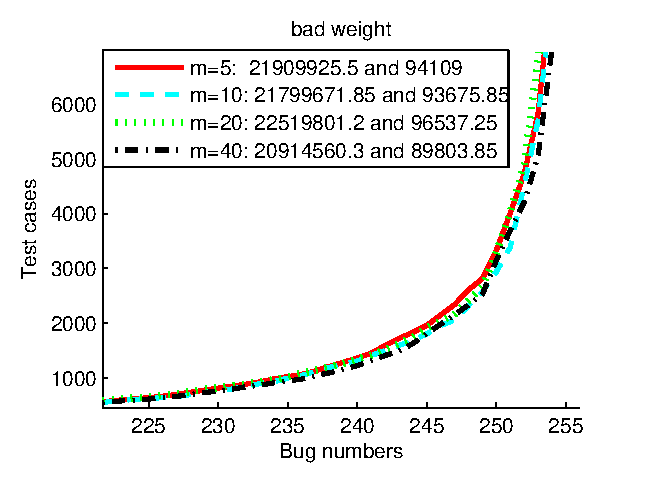
\includegraphics[width=0.45\textwidth]{./a1_picture_enlarge/bad_enlarge.eps}
   \label{fig:bada}
   }
\caption{Algorithm 1:good weight and bad weight(enlarge)}
 \end{figure*}

Figure.\ref{fig:pbad_bugs_testcase} is the case for bad\_weight pair-wise, and
figure.\ref{fig:pbad_bugs_testcase_enlarge} is the enlarged figure. 
From these figures, we can see that best test efficiency is  
$m=5$, and then $m=40,20,10$ using Metric\_1 as well as Metric\_2.  

Table.\ref{table:good_and_bada} also shows the
comparisons between the good\_weight and the 
bad\_weight algorithm for bug\_testcase. From table \ref{table:good_and_bada}, 
we see that at $m=5,10,20,40$, the good\_weight perform better than 
that of bad\_weight algorithm. 

\begin{table*}
    \renewcommand{\arraystretch}{1.2}
    \caption{Algorithm 1:Good and Bad(enlarge),m=5,10,20,40}
    \label{table:good_and_bada}
    \centering
    \begin{tabular}{c c c c c}
    \hline
                                &          m=5            &         m=10           &       m=20            &    m=40   \\ \hline
    \multirow{2}{*}{Good} &  $M_1=23443232.6$    & $M_1=21194024.4$     & $M_1=19752087.8$   & $M_1=19217087.3$ \\
                          &  $M_2=100419.45$     & $M_2=91356.55$       & $M_2=95169.8$      & $M_2=83223.5   $     \\ \hline
    \multirow{2}{*}{Bad}  &  $M_1=21909925.5$    & $M_1=21799671.85$    & $M_1=22519801.2$   & $M_1=20914560.3$ \\
                          &  $M_2=94109$         & $M_2=93675.85$       & $M_2=96537.25$     & $M_2=89803.85 $ \\ \hline 
    \end{tabular}
\end{table*}

We also give the weighted combinatorial coverage as shown in
figure\ref{fig:bcombination_coverage_good},
figure\ref{fig:bcombination_coverage_bad}. 
$i\_{way}$ combinatorial coverage as shown in
figure\ref{fig:bi_ways_combinatio_coverage_good} for good\_weight,
figure\ref{fig:bi_ways_combinatio_coverage_bad} for bad\_weight case,
respectively.

 \begin{figure*}
 %[htb]
   \centering
   \subfloat[Algorithm 1:Combination coverage good(enlarge)]{
   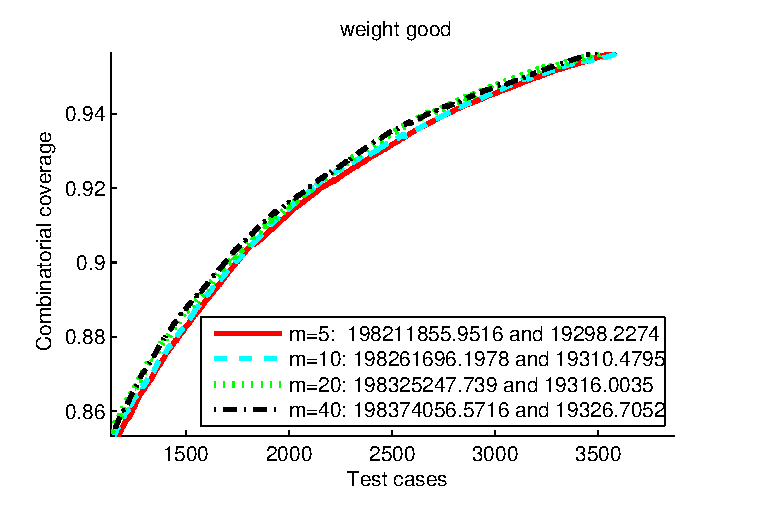
\includegraphics[width=0.45\textwidth]{./a1_picture_enlarge/combination_coverage_good_enlarge.eps}
   \label{fig:bcombination_coverage_good}
   }
   \subfloat[Algorithm 1:Combination coverage bad(enlarge)]{
   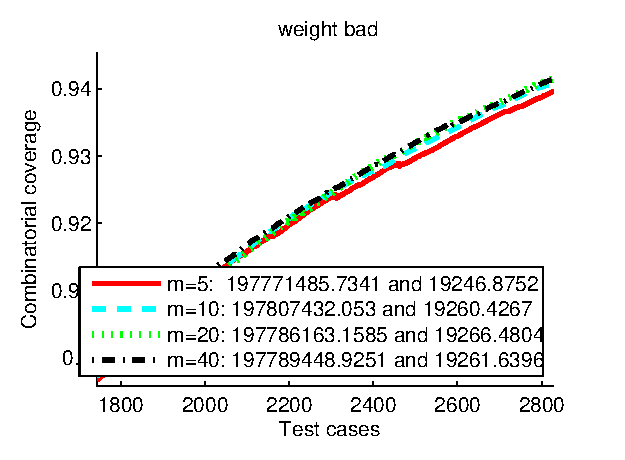
\includegraphics[width=0.45\textwidth]{./a1_picture_enlarge/combination_coverage_bad_enlarge.eps}
   \label{fig:bcombination_coverage_bad}
   }
\caption{Algorithm 1:Combinatorial coverage good and bad enlarge}
\end{figure*}

 \begin{figure*}
 %[htb]
   \centering
   \subfloat[Algorithm 1:i ways combination coverage good(enlarge)]{
   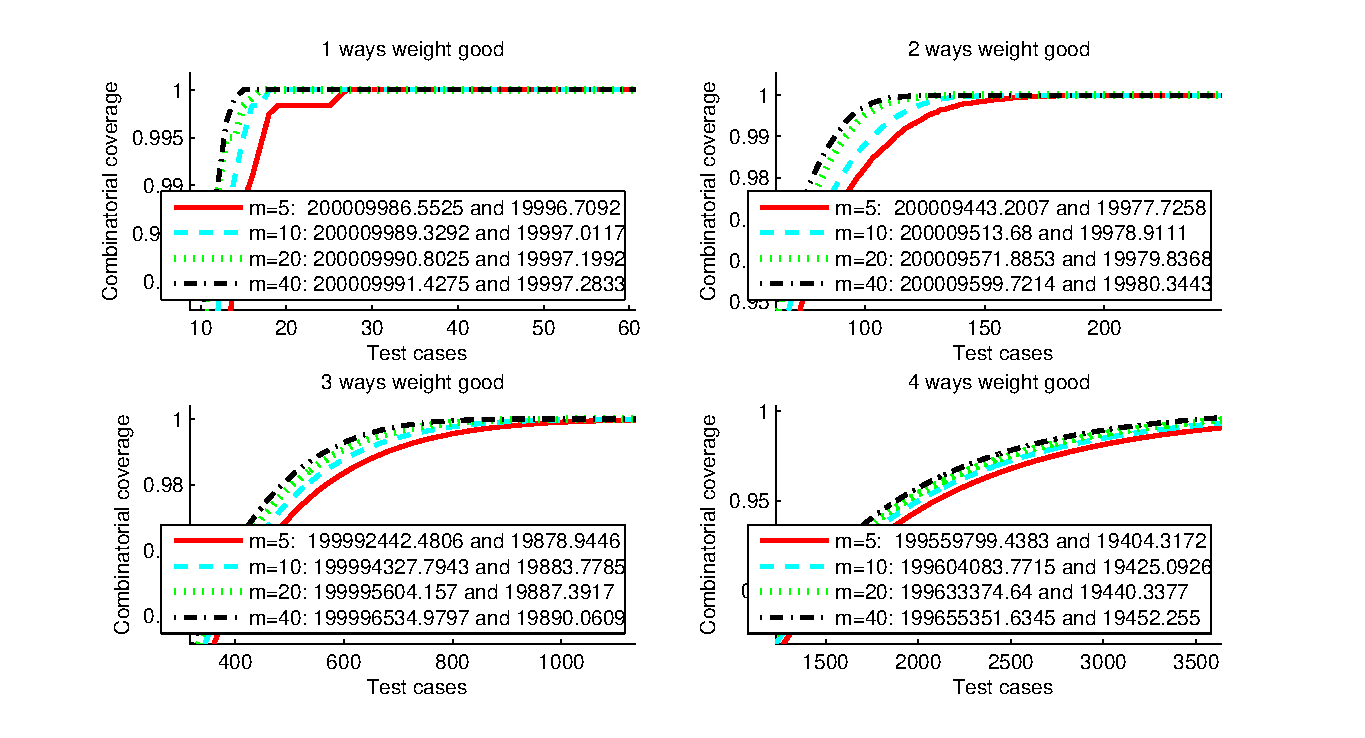
\includegraphics[width=0.45\textwidth]{./a1_picture_enlarge/i_ways_combinatio_coverage_good_enlarge.eps}
   \label{fig:bi_ways_combinatio_coverage_good}
   }
   \subfloat[Algorithm 1:i ways combination coverage bad(enlarge)]{
   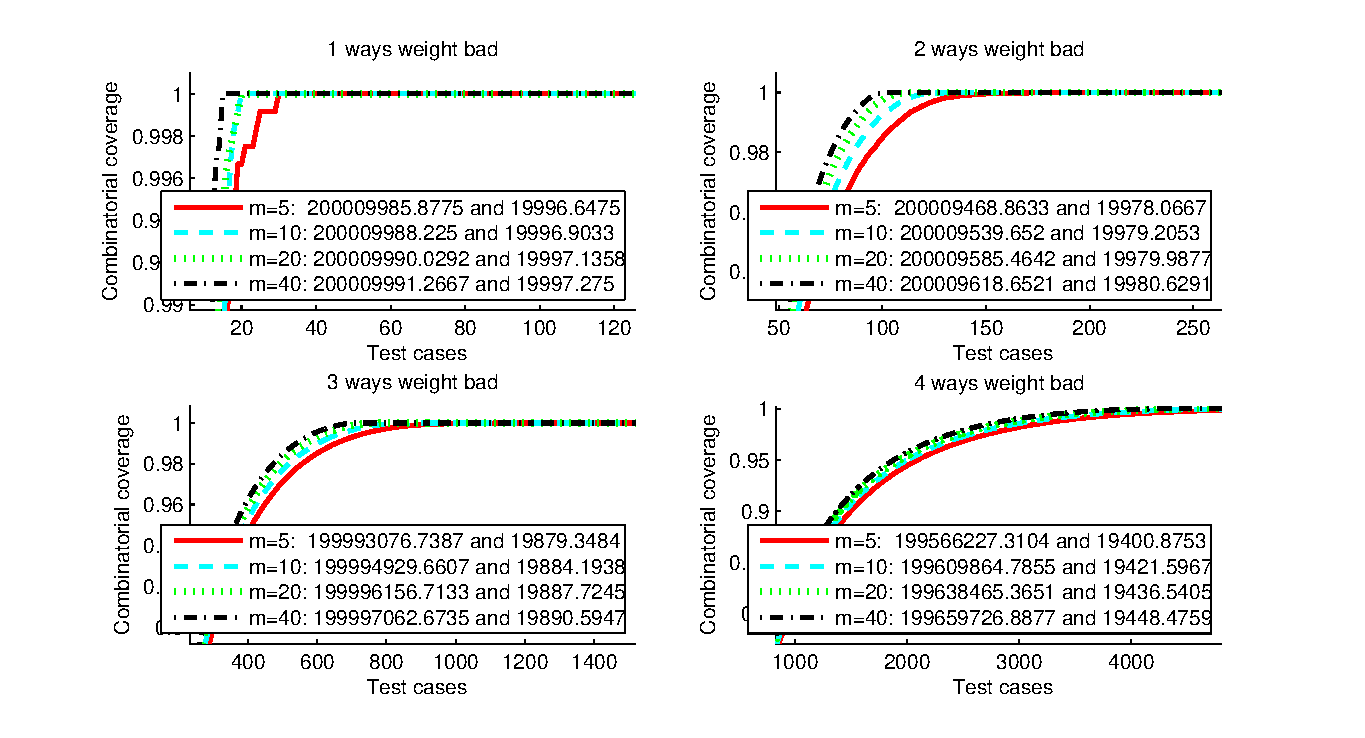
\includegraphics[width=0.45\textwidth]{./a1_picture_enlarge/i_ways_combinatio_coverage_bad_enlarge.eps}
   \label{fig:bi_ways_combinatio_coverage_bad}
   } 
\caption{Algorithm 1:i ways combinatorial coverage good and bad(enlarge)}
\end{figure*}

\section{conclusion}
\label{sec:conclustion}

%\bibliographystyle{ACM-Reference-Format-Journals}
\bibliographystyle{IEEEtran}
\bibliography{IEEEabrv,ctgen_weight}

\end{CJK}
\end{document}
